\documentclass{beamer}
\usetheme{CambridgeUS}
\usecolortheme{beaver}

\usepackage{graphicx}
\usepackage{listings}
\usepackage{xcolor}

% -------- LISTING STYLE --------
\lstset{
    basicstyle=\ttfamily\small,
    keywordstyle=\color{blue},
    commentstyle=\color{green!50!black},
    stringstyle=\color{red},
    breaklines=true,
    frame=single
}

\title{Single-Cycle RISC-V Processor}
\author{Hamza Arif \\ Reg No: 2024206 \\ CE-222L}
\date{\today}

\begin{document}

% ---------------- TITLE ----------------
\frame{\titlepage}

% ---------------- INTRO ----------------
\begin{frame}{Project Overview}
\begin{itemize}
    \item Designed a \textbf{32-bit single-cycle RISC-V processor}
    \item Supports subset of RV32I instructions
    \item Implemented using \textbf{Verilog HDL}
    \item Each instruction executes in \textbf{one clock cycle (CPI = 1)}
\end{itemize}
\end{frame}
\begin{frame}{Processor Architecture}

\begin{columns}

\column{0.35\textwidth}
\centering
\begin{itemize}
    \item Program Counter (PC)
    \item Instruction Memory
    \item Register File
    \item ALU
    \item Data Memory
    \item Control Unit
    \item Immediate Generator
\end{itemize}

\column{0.4\textwidth}
\centering
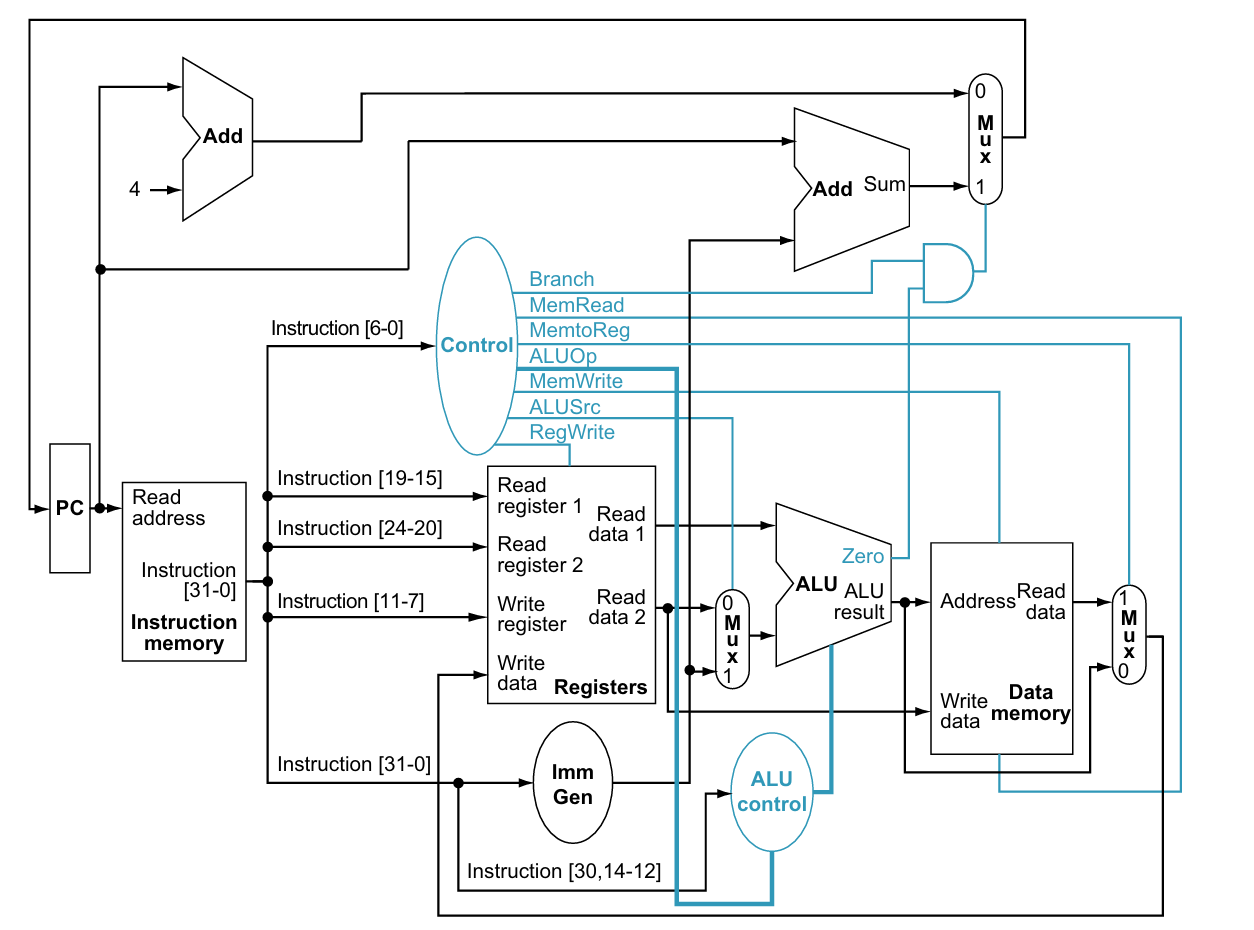
\includegraphics[width=1.25\linewidth]{architecture.png}

\end{columns}

\end{frame}
% ---------------- EXECUTION IDEA ----------------
\begin{frame}{Single-Cycle Execution Idea}
\begin{itemize}
    \item All stages happen in one cycle:
\end{itemize}

\centering
IF $\rightarrow$ ID $\rightarrow$ EX $\rightarrow$ MEM $\rightarrow$ WB

\begin{itemize}
    \item Clock period depends on longest instruction path
\end{itemize}
\end{frame}

% ---------------- EXAMPLE ----------------
\begin{frame}[fragile]{Example: lw Instruction}
\textbf{Instruction:}
\begin{lstlisting}
lw x1, 0(x0)
\end{lstlisting}

\begin{itemize}
    \item Fetch instruction from memory
    \item Decode and read registers
    \item ALU computes address
    \item Memory read
    \item Write back to x1
\end{itemize}
\end{frame}

% ---------------- TEST PROGRAM ----------------
\begin{frame}[fragile]{Test Program}
\begin{lstlisting}
lw  x1, 0(x0)
lw  x2, 4(x0)
add x3, x1, x2
sub x4, x2, x1
sw  x3, 8(x0)
and x5, x3, x4
or  x6, x3, x4
beq x4, x1, 8
32: sw  x1, 12(x0)  # SHOULD BE SKIPPED
36: sw  x2, 16(x0)  
\end{lstlisting}
\end{frame}

% ---------------- SIMULATION RESULTS ----------------
\begin{frame}{Simulation Results}

\centering

\begin{minipage}{0.48\textwidth}
    \centering
    \includegraphics[width=\linewidth]{terminal2.png}

    \vspace{0.2cm}
    \textbf{Register Results}
\end{minipage}
\hfill
\begin{minipage}{0.48\textwidth}
    \centering
    \includegraphics[width=\linewidth]{terminal3.png}

    \vspace{0.2cm}
    \textbf{Memory Results}
\end{minipage}

\end{frame}

% ---------------- INITIAL STATE ----------------
\begin{frame}[fragile]{Execution Trace (Initial State)}
\begin{lstlisting}
All registers = 0
Memory[0] = 10
Memory[4] = 20
\end{lstlisting}
\end{frame}

% ---------------- EXECUTION TRACE ----------------
\begin{frame}[fragile]{Execution Trace (Register Updates)}

\begin{columns}

% -------- LEFT --------
\column{0.5\textwidth}
\begin{lstlisting}
1. lw x1, 0(x0)
   x1 = 10

2. lw x2, 4(x0)
   x2 = 20

3. add x3, x1, x2
   x3 = 30

4. sub x4, x2, x1
   x4 = 10
\end{lstlisting}

% -------- RIGHT --------
\column{0.5\textwidth}
\begin{lstlisting}
5. sw x3, 8(x0)
   Memory[8] = 30

6. and x5, x3, x4
   x5 = 10

7. or x6, x3, x4
   x6 = 30

8. beq x4, x1
   Taken (Jump to 36)
\end{lstlisting}

\end{columns}

\end{frame}

% ---------------- WAVEFORM ----------------
\begin{frame}{Waveform Verification}
\centering
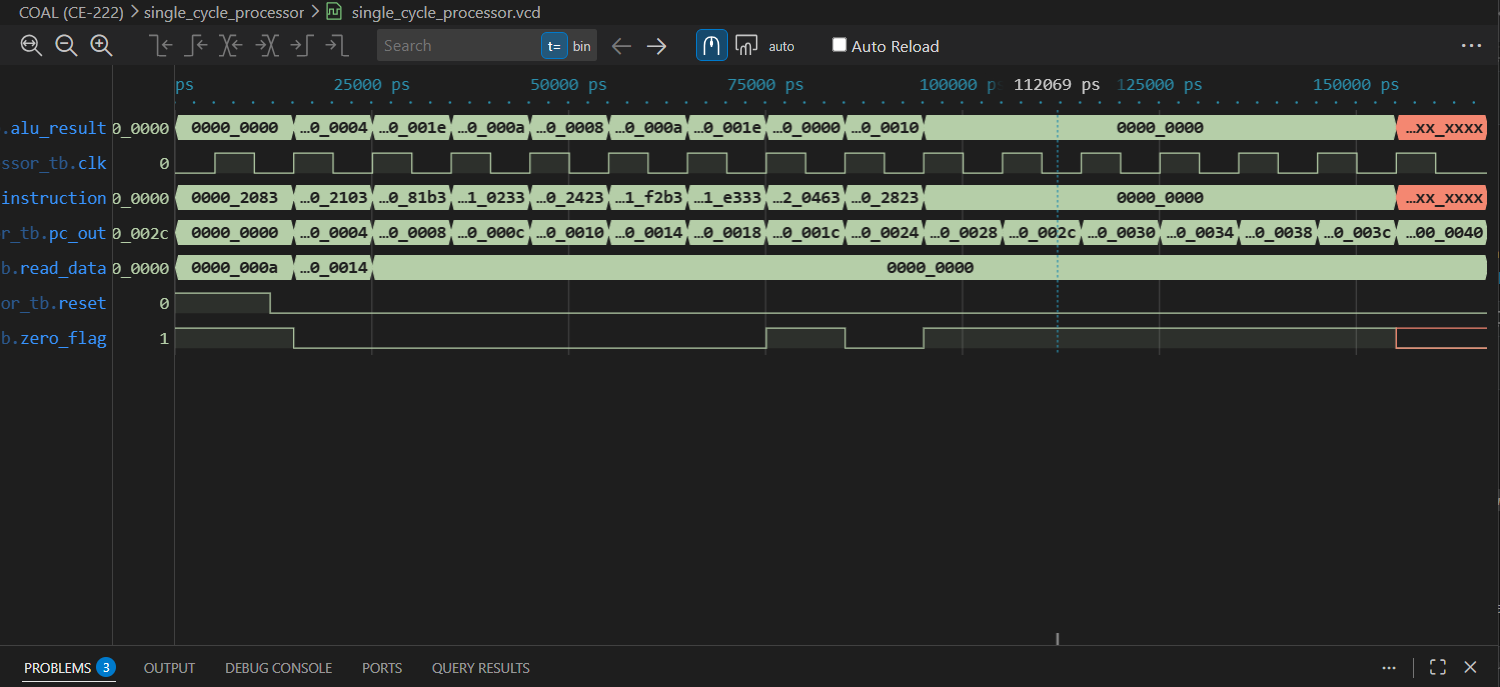
\includegraphics[width=0.85\linewidth]{waveform.png}

\vspace{0.3cm}
\begin{itemize}
    \item Confirms single-cycle execution timing
\end{itemize}
\end{frame}

% ---------------- CONCLUSION ----------------
\begin{frame}{Conclusion}
\begin{itemize}
    \item Successfully implemented a subset of instructions
    \item Verified complete datapath functionality
    \item Demonstrates simple but efficient single-cycle design
\end{itemize}
\end{frame}

% ---------------- END ----------------
\begin{frame}
\centering
\Large Thank You
\end{frame}

\end{document}